\documentclass[conference]{IEEEtran}
\usepackage[printonlyused]{acronym}
\usepackage[english]{babel}
\usepackage[T1]{fontenc}

\usepackage{url}
\usepackage{import}
\usepackage{siunitx}
\usepackage{float}
\usepackage{tocbibind}
\usepackage{booktabs}
\usepackage{cite}
\usepackage{amsmath,amssymb,amsfonts}
\usepackage{graphicx}
\usepackage{xcolor}
\usepackage{hyperref}
\usepackage{dirtree}
\usepackage{multirow}
\usepackage{array}
\usepackage{minted}
\usepackage{verbatim}
\usepackage{lipsum}
%\usepackage{textcomp}
%\usepackage{subcaption}


\graphicspath{{../img/}}
\newcommand{\placeholder}[1]{\color{red}\textit{!#1}}

\begin{document}

\title{Docker's Architecture and Security: an Overview}

\author{
    \IEEEauthorblockN{Raquel Guerra, M10625}
    \IEEEauthorblockA{\textit{Departamento de Informática} \\
        \textit{Universidade da Beira Interior}\\
        Covilhã, Portugal \\
        raquel.guerra@ubi.pt}
}

\maketitle

\begin{abstract}
    Hardware virtualization provides a reliable and secure isolated environment at the cost of the host resources and performance. Therefore, containers have proven to be lightweight while maintaining the bare-metal performance. Docker has become industry standard as it provides an easy to use platform to create and manage container. This paper aims to explore Docker's architecture and the main security and isolation functionalities that allows it to deploy secure and reliable containers.

    %For a long period, ensuring that an application's performance is consistent across multiple, while managing different versions of, programing languages and libraries was almost impossible task. Thus, IT departments started to adopt the use of virtualization.have solved multiple issues regarding portability and compatibility of applications, but also introduced the concept of application isolation, which allowed multiple applications to be executed in parallel in the same machine without the risk of interference between them, by creating multiple  on the same system. However, virtualization has several drawbacks, the biggest one being the performance degradation due to the heavy nature of virtualizing 

    %O abstract tem de ser um resumo muito resumido de “este era o problema, haviam estas soluções, tinham falhas (não precisas dizer quais), e o Docker propõe-se a responder a isso com o uso de containers”. Depois dizes que no artigo são explorados X, Y e Z tópicos sobre o Docker e, por fim, se o Docker é uma solução viável ou não (mais nada)

    % (150 words)
    % For a long period, ensuring that an application's performance is consistent across multiple, while managing different versions of, programing languages and libraries was almost impossible task. Thus, IT departments started to adopt the use of virtualization.have solved multiple issues regarding portability and compatibility of applications, but also introduced the concept of application isolation, which allowed multiple applications to be executed in parallel in the same machine without the risk of interference between them, by creating multiple  on the same system. However, virtualization has several drawbacks, the biggest one being the performance degradation due to the heavy nature of virtualizing an entireor even different architectures. In addition, the need for portability was not fully met with. Hypervisor software from different vendors creates an additional roadblock to deploying applications regardless of the underlying hardware. Therefore, the IT industry has been steadily adopting the use of containerization. Containers provide an lightweight and
    
    % (100 words)
    % For a long period, ensuring that an application's performance is consistent across multiple, while managing different versions of, programing languages and libraries was almost impossible task. Thus, IT departments started to adopt the use of virtualization.have solved multiple issues regarding portability and compatibility of applications, but also introduced the concept of application isolation, which allowed multiple applications to be executed in parallel in the same machine without the risk of interference between them, by creating multiple  on the same system. However, virtualization has several drawbacks, the biggest one being the performance degradation due to the heavy nature of virtualizing 


\end{abstract}

\section*{Acronyms}
\begin{acronym}[REST]
    \acro{API}{Application Programming Interface}
    \acro{CLI}{Command Line Interface}
    \acro{OCI}{Open Container Initiative}
    \acro{OS}{Operating System}
    \acro{REST}{REpresentational State Transfer}
\end{acronym}


\section{Introduction}
\label{sec:intro}

\lipsum[1] THIS IS A \ac{2FA}\cite{Kane2018-fn}.

\section{Docker Architecture}
\label{sec::arch}

\placeholder{Architecture intro}

% 3. Docker Architecture
%     1. The Docker engine
%         1. Client server
%         2. Monolithic architecture
%         3. runc
%         4. containerd
%     2. Images
%         1. Layers
%         2. Dockerfile
%         3. Docker compose
%     3. Containers
%         1. Container creation process
%         2. Workflow
%     5. Volumes and persistent data
%     6. Networking

% TODO:
% explain libcontainer

\subsection{The Docker Engine}
\label{sec::arch:engine}
The Docker Engine is the core software responsible for running and managing containers, which consists of several modular components\cite{Docker-engine}. It is implemented as a client-server application, consisting of:

\begin{itemize}
    \item A server running the daemon process \texttt{dockerd};
    \item Docker's \acs{REST}ful \acs{API};
    \item The \acs{CLI} client, \texttt{docker}.
\end{itemize}

Within this architecture, the Docker daemon is the component responsible for creating, running and managing the containers. The daemon is able to manage any number of containers in the device, all controlled via the \acs{CLI} client. The client interacts with the Docker daemon via its own \acs{REST} \acs{API} over Unix sockets or a network interface\cite{Poulton2020-ju}.

\begin{figure}[!htb]
    \centering
    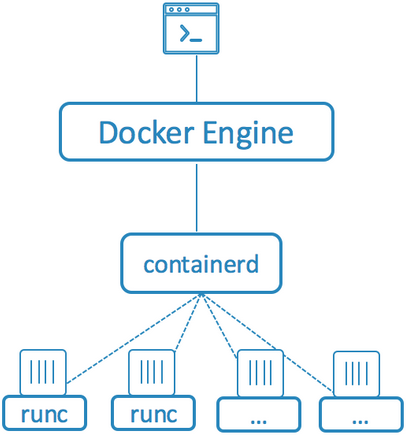
\includegraphics[width=0.25\textwidth]{docker_engine.png}
    \caption{Current and planned container use for all organizations.}
    \label{fig:docker-engine-server}
\end{figure}

Despite being, at its core, a client-server architecture, Docker's server is far from monolithic, as shown in figure \ref{fig:docker-engine-server}. The server operates a set of smaller components, among them \texttt{runc} and \texttt{containerd}, the main modules responsible for creating and running containers. Both implement as closely as possible the OCI open source project specifications\cite{Poulton2020-ju, oci-runc, git-runc, docker-containerd}.

The first program, \texttt{runc}, is a \acs{CLI} component responsible for creating and running applications. Its purpose is to be a standalone low-level tool called by any high-level application, such as Docker. In order to achieve this, \texttt{runc} relies on the library \texttt{libcontainer} to access the container isolation features of the \acs{OS}, such as \texttt{seccomp} and user namespaces\cite{runc-estes}.

Secondly, \texttt{containerd} is responsible for managing all the container execution logic, such as starting, stopping and removing containers. In the same way as \texttt{runc}, \texttt{containerd} is available as a standalone daemon and was intended to be a lightweight program with the sole role of managing container lifetime operations. But as it grew, it gained new functionalities, such as data storage and image management\cite{docker-containerd}.

With this in mind, it's possible to understand the container creation workflow. When a command is typed in the \acs{CLI}, the Docker client converts the instructions into the \acs{API} payload and POSTs to the correct API endpoint. Once the daemon receives the command to create a new container, a call is made to \texttt{containerd}, which converts the required Docker image into a bundle and instructs \texttt{runc} to create a new container. In its turn, \texttt{runc} interfaces with the \acs{OS} kernel to allocate the resources and to execute the instructions needed to create a new container. The container process is started as a child-process of \texttt{runc}, and as soon as it is started, \texttt{runc} is terminated.


\subsection{Containers}
\label{sec::arch:containers}
As defined by the \texttt{libcontainer} README page, a container is "a self-contained execution environment that shares the kernel of the host system and is optionally isolated from other containers in the system"\cite{docker-libcontainer}.

Despite the behavior similarities between containers and \acsp{VM}, they are fundamentally different since all the containers running in the system share the same kernel, so the isolation between workloads is implemented within that one kernel. As a result, there is one less layer of abstraction between the isolated task and the hardware underneath, which results in better resource efficiency.

However, it's only possible to run processes that are compatible with the underlining kernel, \ie~ a Windows container cannot run Linux application and vice versa.

% \subsection{Container Lifecycle}
% \placeholder{Dockerfile}
% 
% \placeholder{docker compose}
% containers follow the same process group signal propagations that any other process group would recieve on linux
% auto restarting a continer?
% normal docker stop sends a SIGTERM to kill the container
% docker stop initially sends sigterm signal, if the container as not stopped within 25 seconds, a SIGKILL signal is sent to forcefully kill it
% if docker kill wont stop the container, docker kill is used

% The Dockerfile has two main purposes:
% 1. To describe the application
% 2. To tell Docker how to containerize the application (create an image with the app inside)

\subsection{Images}
\label{sec::arch:images}
Docker images are a template of what is reconstructed into a running container, it serves as a base for everything that will be deployed and run on the container, similarly to a filesystem \cite{Kane2018-fn}. Before launching a container, the image must be built from scratch or downloaded from a public registry. When the \texttt{docker pull} command is used, the default registry used is the official Docker Hub \cite{docker-hub}.

An image consists of multiple read-only layers; each layer represents the changes made to the underlining system, \ie~ a \texttt{diff} of the previous layer \cite{images-layers}. When a container is created, a new read-write layer is added on top of the previous ones, so that all the changes made during the container execution are saved on disk (figure \ref{fig:docker-image}) \cite{fig-src:image-layers}.

A layer is identified by a digest, referred to as \textit{Content Addressable IDs}, as each hash represents the image content. This model of layer separation allows several images to address the same layer. As such, the latter only needs to be stored once in the device.

\begin{figure}[!htb]
    \centering
    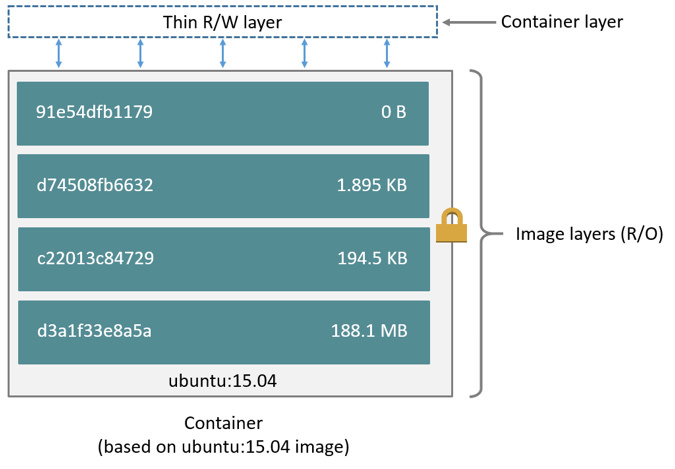
\includegraphics[width=0.45\textwidth]{container-layers.jpg}
    \caption{Diagram exemplificative of a Docker image composition, where the set of layers composes an Ubuntu container \cite{fig-src:image-layers}.}
    \label{fig:docker-image}
\end{figure}

These layers are described in the image manifests, which are \acs{JSON} files containing both information about the image's layers and a list of compatible architectures given by an image tag \cite{image-manifest}.

\placeholder{Use image storage driver to connect to next section}
% https://docs.docker.com/storage/storagedriver/

\subsection{Volumes and persistent data}
\label{sec::arch:volumes}

When a container is created, the system automatically allocates local storage where the container's filesystem is stored. However, this integral part of the container is tied to it's lifecycle, it will be deleted as soon the container itself is deleted. By default, the container uses only this local storage. If persistent storage is needed, there are two options for containers to store data on the host device: volumes and bind mounts\cite{container-storage}.

Volumes are created and managed by Docker and are stored within a folder on the host machine. As volumes are only managed by Docker, this means they are isolated from the host and only Docker is allowed to write any change made to the volume. It's possible to mount a single volume into multiple containers. When a given volume isn't being used by any container it won't be removed automatically.

On the other hand, bind mounts consist on directories on the host machine being mounted into a container. This mounts are limited in functionality, as they are not managed by Docker itself.

\placeholder{Connect section to Networking, if possible}

\subsection{Networking}
\label{sec::arch:net}

Different types of bridge networking:

\begin{itemize}
    \item bridge
    \item host
    \item overlay
    \item macvlan
\end{itemize}


\section{Docker Security}
\label{sec::security}

% 4. Docker security
%     1. UID 0
%     2. Privileged Containers
%     3. Secure Computing Mode
%     4. SElinux and AppArmor

\placeholder{Begin draft}
\subsection{cgroups}
\label{ssec::security:cgroups}
fundamental building blocks that are used to make containers: control groups,

Cgroups limit the resources, such as memory, CPU, and network input/output, that a group of processes can use. From a security perspective, well-tuned cgroups can ensure that one process can't affect the behavior of other processes by hogging all the resources

Docker automatically creates its own cgroups of each type.

When you start a container, it automatically creates another set of cgroups within the docker cgroups. Create a container and give it a memory limit that we can observe within the memory cgroup.

Constraining resources provides protection against a class of attacks that attempt to disrupt your deployment by consuming excessive resources, thereby starving legitimate applications. It's recommended that you set memory and CPU limits when you run your container applications.

\subsection{Namespaces}
\label{ssec::security:namespaces}

Kernel namespaces are at the very heart of containers! They let us slice up an operating system (OS) so that it looks and feels like multiple isolated operating systems.

namespaces control what it can see. By putting a process in a namespace, you can restrict the resources that are visible to that process.

Unix systems allowed the mounting of filesystems, but they would all be mounted into the same system-wide view of all filenames. In Plan 9, each process was part of a process group that had its own “name space” abstraction, the hierarchy of files (and file-like objects) that this group of processes could see. Each process group could mount its own set of file systems without seeing each other.

There are several different kinds of namespace supported by Linux:
\begin{itemize}
    \item Unix Timesharing System (UTS)—this sounds complicated, but to all intents and purposes this namespace is really just about the hostname and domain names for the system that a process is aware of.
    \item Process IDs
    \item Mount points
    \item Network
    \item User and group IDs
    \item Inter-process communications (IPC)
    \item  Control groups (cgroups)
\end{itemize}

Let's briefly look at how Docker uses each namespace:
\begin{itemize}
    \item Process ID namespace: Docker uses the pid namespace to provide isolated process trees for each container. Every container gets its own process tree, meaning that every container can have its own PID 1. PID namespaces also mean that a container cannot see or access to the process tree of other containers, or the host it's running on.
    \item Network namespace: Docker uses the net namespace to provide each container its own isolated network stack. This stack includes; interfaces, IP addresses, port ranges, and routing tables. For example, every container gets its own eth0 interface with its own unique IP and range of ports.
    \item Mount namespace: Every container gets its own unique isolated root / filesystem. This means that every container can have its own /etc, /var, /dev etc. Processes inside of a container cannot access the mount namespace of the Linux host or other containers — they can only see and access their own isolated mount namespace.
    \item Inter-process Communication namespace: Docker uses the ipc namespace for shared memory access within a container. It also isolates the container from shared memory outside of the container.
    \item User namespace: Docker lets you use user namespaces to map users inside of a container to different users on the Linux host. A common example is mapping the root user of a container to a non-root user on the Linux host.
    \item User namespaces are quite new to Docker and currently optional. This may change in the future.
    \item UTS namespace: Docker uses the uts namespace to provide each container with its own hostname.  By putting a process in its own UTS namespace, you can change the hostname for this process independently of the hostname of the machine or virtual machine on which it's running The container can have its own hostname because Docker created it with its own UTS namespace
\end{itemize}

\subsection{UID 0}
\label{ssec::security:uid0}

The user namespace allows processes to have their own view of user and group IDs. Much like process IDs, the users and groups still exist on the host, but they can have different IDs. The main benefit of this is that you can map the root ID of 0 within a container to some other non-root identity on the host. This is a huge advantage from a security perspective, since it allows software to run as root inside a container, but an attacker who escapes from the container to the host will have a non-root, unprivileged identity.

User namespaces allow an unprivileged user to effectively become root within the
containerized process. This allows a normal user to run containers using a concept called rootless containers, The general consensus is that user namespaces are a security benefit because fewer containers need to run as “real” root

\subsection{Privileged Containers}
\label{ssec::security:priv-cont}

\placeholder{TODO}

\subsection{Secure Computing Mode}
\label{ssec::security:sec-compt}
\placeholder{TODO}

\subsection{Mandatory Access Control}
\label{ssec::security:sel-apparm}

Using mandatory access controls gives the administrator much more granular control of what can happen on their system, in a way that individual users can't override.

\subsubsection{\textbf{AppArmor}}
AppArmor (short for “Application Armor”) is one of a handful of Linux security
modules (LSM) that can be enabled in the Linux kernel. In AppArmor, a profile can be associated with an executable file, determining what that file is allowed to do in terms of capabilities and file access permissions. AppArmor and other LSMs implement mandatory access controls. A mandatory access control is set by a central administrator, and once set, other users do not have any ability to modify the control or pass it on to another user.

AppArmor includes a “complain” mode in which you can run your executable against a profile and any violations get logged. The idea is that you can use these logs to update the profile, with the goal of eventually seeing no new violations, at which point you start to enforce the profile.

\subsubsection{\textbf{SELinux}}
SElinux lets you constrain what a process is allowed to do in terms of its interactions with files and other processes. Each process runs under an SELinux domain—you can think of this as the context that the process is running in—and every file has a type.

A key distinction between SELinux permissions and regular DAC Linux permissions is that in SELinux, permissions have nothing to do with the user identity—they are described entirely by labels. That said, they work together, so an action has to be permitted by both DAC and SELinux.

Creating an effective SELinux profile for an application takes in-depth knowledge of the set of files that it might need access to, in both happy and error paths, so that task may be best left to the app developer. Some vendors provide profiles for their applications.



\placeholder{End draft}
\section{Conclusion}
\label{sec::conc}

% Abriste o artigo com o problema do hardware dedicado a uma aplicação e das VMs. Apresentaste o Docker como um software que se propõe a responder a este problema. Na conclusão diz se o Docker de facto resolve o problema ou não, quais os problemas e limitações actuais dele que identificas, e, caso exista, qual o roadmap do Docker para colmatar essas limitações

% FROM ABSTRACT: Henceforth, Docker is a robust solution for the deployment of multiple real-world applications while better taking advantage of available resources and Linux kernel native functionalities and security model.






\bibliography{../bibtex/bibliography}
\bibliographystyle{../bibtex/IEEEtran}

\end{document}